\documentclass[
  lualatex,
  aspectratio=169,
  fleqn,
  14pt,
]{beamer}
\batchmode

\usetheme[progressbar=frametitle]{Metropolis}
\setbeameroption{show notes on second screen=bottom}

\usepackage{xparse}
\usepackage{mathtools,amssymb}
\usepackage{graphicx,xcolor}
\usepackage{pxrubrica}
\usepackage{calc}
\usepackage[absolute,overlay]{textpos}
%\usepackage{enumitem}
\usepackage[1.7]{bxpdfver}
\usepackage{pdfcomment}
\usepackage{ulem}
\usepackage{stackengine}
\usepackage{appendixnumberbeamer}
\usepackage{tabto}
\usepackage[superscript]{cite}

\RenewDocumentCommand\citeform{m}{[#1]}

% フォント
\usepackage[lining,tabular,sfdefault]{FiraSans}
\usepackage[mathrm=sym,mathbf=sym]{unicode-math}
\setmathfont{Fira Math}
\usepackage[no-math,deluxe,haranoaji]{luatexja-preset}
\RenewDocumentCommand\kanjifamilydefault{}{\gtdefault}

% 打ち消し線関連
\RenewDocumentCommand\ULthickness{}{.1\zh}
% 二重打ち消し
\NewDocumentCommand\dsout{m}{%
  \stackengine{.2\zh}{#1}{%
    \stackengine{-.3\zh}{\sout{\hphantom{#1}}}{\sout{\hphantom{#1}}}{O}{c}{F}{F}{L}%
  }{O}{c}{F}{F}{L}}

% 下に文字置くやつ
\NewDocumentCommand\replace{mm}{%
  \smash{\stackengine{-1\zh}{\dsout{#1}}{#2}{O}{c}{F}{F}{L}}}

% 床関数
\DeclarePairedDelimiter\floor\lfloor\rfloor

\usepackage{hyperref}

\title{郵便を用いた超低速IP通信システムの検討}
\subject{エンジニア作業飲み集会\#XXX}
\author{%
  \texorpdfstring{%
    \ltjsetparameter{autospacing=false, autoxspacing=false}
    上羽 未栞\inst{\dag}\inst{a)}\and
    信濃 眞伊\inst{\dag}\inst{b)}\and
    佐伯 真紘\inst{\dag}\inst{c)}\and
    一式 すみれ\inst{\dag}\inst{d)}}
    {上羽 未栞\and 信濃 眞伊\and 佐伯 真紘\and 一式 すみれ}}
\institute{
  \inst{\dag}\hspace{.66\zw}東京広域電話網, \url{https://tkytel.github.io/}\\
  a) a.k.a. KusaReMKN, \url{mkn@kusaremkn.com}\\
  b) \url{me@shinanomai.xyz}\\
  c) a.k.a. Nejikugi, \url{me@scrwnl.eu.org}\\
  d) a.k.a. yude, \url{i@yude.jp}
}
\keywords{LoLLIPoP; 郵便; TCP/IP; RFC 1149}
\date{2025-11-07}

\begin{document}

\begin{frame}
  \titlepage
  \thispagestyle{empty}
  \note{
    はじまるよ〜。

    郵便を用いた超低速IP通信システムの検討と題して、
    東京広域電話網のLoLLIPoPチームを代表して
    上羽未栞が発表するよ。
  }
\end{frame}

\begin{frame}
  \frametitle{今回のおはなし}

  ~\\[.25\baselineskip]
  \tableofcontents
  \note{
    今回の発表の流れはこんな感じだよ。
    おおよそ25分くらいで進められたらいいな。
  }
\end{frame}

\section*{みかんちゃんについて}
\note{
  まずは自己紹介するよ〜。
}

\begin{frame}
  \frametitle{自称・大天才美少女プログラミング初心者}

  \begin{textblock*}{0.5\paperwidth}(-0.3cm, 3.3cm)
    \includegraphics[width=0.35\paperwidth]{./images/mikanchan.png}
  \end{textblock*}
  \begin{columns}
    \begin{column}{0.30\textwidth}
      \\~\\[-.25\baselineskip]
    \end{column}
    \begin{column}{0.69\textwidth}
      \\~\\[-.25\baselineskip]
      「\ruby{上羽}{うわ|ば} \ruby{未栞}{み|かん}」
      あるいは「\ruby[g]{KusaReMKN}{くされみかん}」\\
      \hspace{1.5\zw}\textbf{みかんちゃん}って呼んでね!
      \\~\\[-.5\baselineskip]

      17{\scriptsize(18)}歳のJK(超重要)\\
      \hspace{1.5\zw}実はプログラマでもエンジニアでもない\\
      \hspace{1.5\zw}普段はホラを吹いて生活している\\
      \hspace{1.5\zw}古い計算機っぽいものが大好き
      \\~\\[-.5\baselineskip]

      Twitterで思想を垂れ流すことが得意\\
      \hspace{1.5\zw}\url{https://kusaremkn.com/}も見てね
    \end{column}
  \end{columns}
  \note{
    自称大天才美少女プログラミング初心者の上羽未栞だよ。
    みかんちゃんって呼ばれると大変喜ぶよ。

    イチナナ歳のJKだよ。重要だよ。
    大天才とか偉ぶっているけれど、実はプログラマでもエンジニアでもないよ。
    普段はホラ吹きを生業としているよ。
    古い計算機っぽいものが大好きで、いろいろなものに手を出しては
    それに掛けられた呪いを解くことを趣味にしているよ。

    Twitterや自分のウェブサイトで思想を垂れ流すのが得意だよ。
    暇な人は眺めてみてね。
  }
\end{frame}

\section{インターネットを支える技術}
\note{
  まずはインターネットを支える技術について思いを馳せてみるよ。
}

\begin{frame}
  \frametitle{インターネットなしでは生きられない!}

  身の周りにある便利なもの
  \begin{itemize}
    \item
      TwitterやYouTubeを支えているWeb
    \item
      しゃべる洗濯機や冷蔵庫を支えているIoT
    \item
      睡眠時間を奪い心身の健康を蝕むVRChat
  \end{itemize}
  全てネットワークを使った通信のおかげ

  \vspace{\zh}
  それなのに……\\
  \hspace{1.5\zw}ネットワークがなぜ繋がるのかあまり考えていない\\
  \hspace{1.5\zw}ネットワークの通信にタダ乗りしているだけ\\

  \note{
    現代社会においては、
    あらゆるものがネットワークに接続されていて、
    何かしら通信していることが常になってきているよ。
    よく例として挙げられるものではWebがあるし、
    最近ではIoTなんかも生活の一部に感じられるようになってきたよ。
    今お前らがこうやってVRChatをしていられるのもネットワークのおかげだよ。
    いわんや、ネットワークを用いた通信は当然のものになっているよ。

    しかし、これを支える技術、
    特により物理側に近い層については関心を寄せる人は
    あまり多くないような印象があるよ。
    これは由々しき事態であるから、
    積極的にネットワークに思いを馳せていきたいね。
  }
\end{frame}

\begin{frame}
  \frametitle{インターネットのしくみ\cite{RFC1122}}

  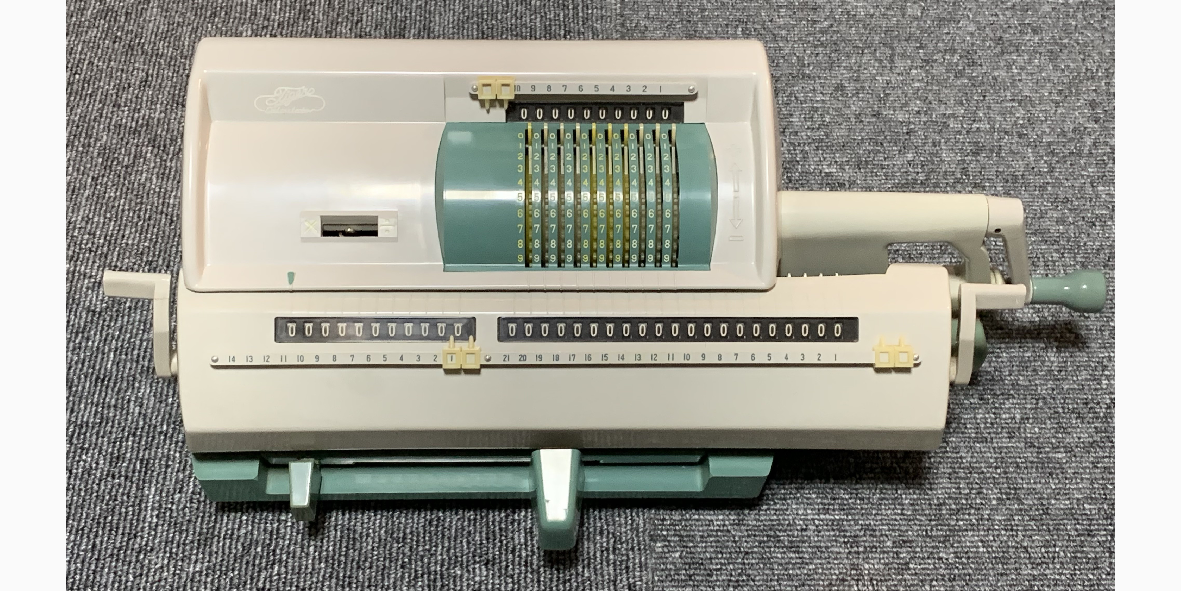
\includegraphics[page=1,width=\linewidth]{./images/pictures.pdf}

  \note{
    ネットワークの代表格であるとろの
    インターネットの基本原理について立ち返るよ。
    TCP/IPでは、より上位から順に、
    アプリケーション層、トランスポート層、インターネット層、リンク層の
    4つの階層から成っているよ。

    アプリケーション層は、例えばWebやVRChatといったサービス、
    名前解決やアドレス自動割り当てなどの機能を実現するよ。
    トランスポート層は、Webのデータをブラウザへ、
    VRChatのデータをVRChatへといった具合に
    適切な通信を適切なアプリケーションに届けるよ。
    インターネット層では、世界中を張り巡らされた数多のネットワークを通り抜け、
    目的のホスト(コンピュータ)までデータを届けるよ。
    リンク層では、そのホストから物理的に直接通信できる範囲でデータを届けるよ。

    これらの層が連携して仕事をすることで様々な通信を実現できるよ。
  }
\end{frame}

\begin{frame}
  \frametitle{情報を伝える根幹のしくみ}

  \includegraphics[page=2,width=\linewidth]{./images/pictures.pdf}

  \note{
    今回のお話では、これらの層の一番下位の部分、リンク層に着目するよ。

    リンク層で用いられるプロトコルとして、
    LANケーブルに電気を通したり、光ファイバに光を通したりして
    通信するEthernetや電波を遣って通信をするWi-Fiなどがあるよ。
    また、少し古めかしいところではダイヤルアップ通信
    (電話線とモデムとを使ったPPP)もリンク層の通信だよ。
    この場合、コンピュータは電話を使って「直接」通信していることになるよ。

    TCP/IPでは下位の層は上位の層にデータを受け渡せれば良いよ。
    つまり、リンク層では、同一リンク内で通信でき、
    適切にデータを伝送できれば良いので、
    ここで用いる伝送方式はかなり自由に選択できるよ。
    「味のあるリンク」で当たり前の通信を実現できると面白そうだね。
  }
\end{frame}

\section{鳥類キャリアによるIP通信}
\note{
}

\begin{frame}
  \frametitle{RFC 1149: 1990年4月1日発のジョークRFC}

  鳥類キャリアを用いたIP通信の手法が検討されている\cite{RFC1149}\\
  \hspace{1.5\zw}QoSの提供\cite{RFC2549}やIPv6への対応\cite{RFC6214}など改良・拡張されている


  \note{
    鳥類キャリア、要は伝書鳩を用いて
    IPデータグラムをカプセル化する手法が検討されているよ。
    この手法は1990年に提案されたものだけど、
    その後も改良や拡張が進められていて、
    QoS(Quality of Service)の提供やIPv6への対応なども提案されているよ。
  }
\end{frame}

\section{郵便を利用したIP通信}

\section{実装・実験}

\section{まとめ・検討事項}

\appendix

\begin{frame}[standout]
  おわりです

  \note{
    おわりだよ〜。
  }
\end{frame}

\begin{frame}
  \frametitle{参考資料}

  \beamertemplatetextbibitems
  \setbeamerfont{bibliography item}{size=\footnotesize}
  \setbeamerfont{bibliography entry}{size=\footnotesize}
  \setbeamerfont{bibliography entry author}{size=\footnotesize}
  \setbeamerfont{bibliography entry title}{size=\footnotesize}
  \setbeamerfont{bibliography entry location}{size=\footnotesize}
  \setbeamerfont{bibliography entry note}{size=\footnotesize}
  \begin{thebibliography}{1}
    \bibitem{RFC1122}
      Braden, R.,
      \newblock
      Requirements for Internet Hosts --- Communication Layers\textmd,
      \newblock
      \href{https://doi.org/10.17487/RFC1122}{RFC 1122}, October 1989.

    \bibitem{RFC1149}
      Waitzman, D.,
      \newblock
      Standard for the transmission of IP datagrams on avian carriers\textmd,
      \newblock
      \href{https://doi.org/10.17487/RFC1149}{RFC 1149}, April 1990.

    \bibitem{RFC2549}
      Waitzman, D.,
      \newblock
      IP over Avian Carriers with Quality of Service\textmd,
      \newblock
      \href{https://doi.org/10.17487/RFC2549}{RFC 2549}, April 1999.

    \bibitem{RFC6214}
      Carpenter B., Hinden  R.,
      \newblock
      Adaptation of RFC 1149 for IPv6\textmd,
      \newblock
      \href{https://doi.org/10.17487/RFC6214}{RFC 6214}, April 2011.
  \end{thebibliography}
\end{frame}

\begin{frame}
  \frametitle{このスライドについて}

  Written in November 2025.

  Permanent ID of this document: \texttt{2976cf5d5f923407}.

  Copyright © 2025 KusaReMKN.

  特記無き場合、プログラムやソースコードは MIT License で、\\
  \hspace{1.5\zw}それ以外のコンテンツは CC-BY 4.0 で利用可能です。\\
  \hspace{1.5\zw}一部の画像には別のライセンスが適用されるかもしれません。
\end{frame}

\end{document}
% ex: se et ts=2 :
